\chapter{Methodology}
% This chapter is for going over my methods and talking about my software architecute and why it looks the way it does.

\section{Research Design} 
\paragraph{}
This thesis is a mixture of both research and design implementation.
The research portion of this project focused on linking an existing C++ application (CuraEngine) into a larger JavaEE based project.
In this research we also had a small group of people run though some beta testing of the application and logged their observations.

%Diagram of how the user interacts with WebSlicer from a high level .
\begin{figure}[!ht]
  \centering
  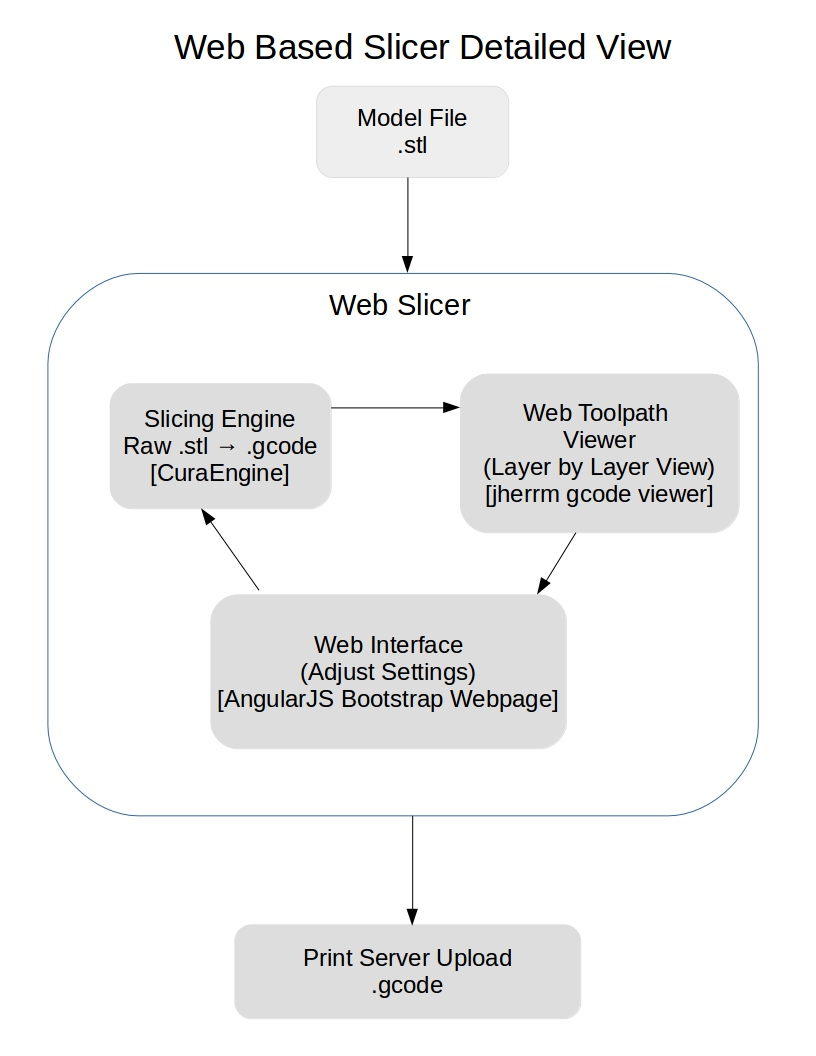
\includegraphics[width=\linewidth]{slicer-detailed-view}
  \caption{High level view of how WebSlicer functions and how users will interact with it}
  \label{fig:slicer-detailed-view}
\end{figure}

\section{Working procedure}
\paragraph{}
% this needs way more info
As shown in Figure \ref{fig:slicer-detailed-view}, the application will have 3 major components that all need to work together in a cycle until the user decides that the output is what they desire.

\subsection{Web Interface}
\paragraph{}
%update this to final version. no more "i anticipate"
I anticipate that it will include a set of forms for collecting the users settings for their printer and account tracking info so that they may retain certain settings. 
Additionally, I would like to include a gcode editor which will allow users to edit specific portions of their gcode and see the resulting output in the viewer. 
This does not include the actual slicing engine which must be driven and accessed independently.

\subsection{Slicing Engine}
\paragraph{}
The slicing engine is at the heart of this project. 
It will include taking uploaded .stl model files by the user and convert them into raw G-code. 
The engine that carries out the raw geometry calculations is CuraEngine and is written in pure C++, (it is not web friendly). 
Thus, this portion of the project will require deploying CuraEngine at a cloud provider and then creating a RESTful API to interface with it.

\subsection{Web Tool Path Viewer}
\paragraph{}
%expand this with more detail
After configuring and generating the G-code representation for a 3D model, there still must be a way to review visually how the slicing engine actually will split up the model. 

\subsection{Final Steps}
\paragraph{}
The final step in the process of this application will be creating links to the finished files where the user can either choose to download the completed G-code file. 
If the user has access to a print server such as OctoPrint, they may opt to copy/paste the link to it where it will be uploaded automatically for printing using the OctoPrint API.

\section{Review and Usability Testing}
\paragraph{}
After running through all steps of the working procedure it was then necessary to test WebSlicer by running a small beta test. 
This beta test consisted of a small group of users with varying familiarity with 3D printing to test how easy WebSlicer is to use through a series of simple tasks.
